% Generated by thesis/ch7/exp1/make_figures.py -- do not edit by hand.
\begin{figure}[tbp]
  \centering
  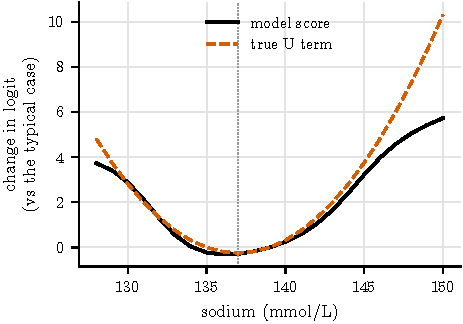
\includegraphics[width=\textwidth,height=0.8\textheight,keepaspectratio]{figures/ch7/options/synthetic-shape-c-sig-best-g300-sodium}
  \caption{Synthetic data (U and saddle), the best sigmoid-unit seed at generation 300 (not explained): response to sodium. Black: the model's score as sodium varies, every other input at the typical case, relative to the typical sodium; dashed: the true U term $((z_n - (-0.5))^2 - 1)$, lowest at 137 mmol/L; dotted: 137 mmol/L.}
  \label{fig:ch7-synthetic-shape-c-sig-best-g300-sodium}
\end{figure}
